\documentclass[conference]{IEEEtran}
\IEEEoverridecommandlockouts
% The preceding line is only needed to identify funding in the first footnote. If that is unneeded, please comment it out.
\usepackage{cite}
\usepackage{amsmath,amssymb,amsfonts}
\usepackage{algorithmic}
\usepackage{graphicx}
\usepackage{textcomp}
\usepackage{xcolor}
\usepackage{float}
\def\BibTeX{{\rm B\kern-.05em{\sc i\kern-.025em b}\kern-.08em
    T\kern-.1667em\lower.7ex\hbox{E}\kern-.125emX}}
\begin{document}

\title{Assignment 2\\
\thanks{Identify applicable funding agency here. If none, delete this.}
}

\author{\IEEEauthorblockN{1\textsuperscript{st} Noah Fredriksen}
\IEEEauthorblockA{\textit{Department of physics and technology} \\
\textit{UiT}\\
Tromsø, Norway \\}
\and
\IEEEauthorblockN{1\textsuperscript{st} Given Name Surname}
\IEEEauthorblockA{\textit{dept. name of organization (of Aff.)} \\
\textit{name of organization (of Aff.)}\\
City, Country \\
email address or ORCID}
}
\maketitle

\section{Task 1}

For all sections in this task, we choose 
\newline

$A^T=$
\begin{bmatrix}
1 & 4 & 2\\
3 & 1 & 5
\end{bmatrix}
\newline

and 
\newline
$b=$
\begin{bmatrix}
1\\
4\\
2
\end{bmatrix}

\subsection{a)}

We have the normal equation 

\begin{equation}
    A^TAx=A^Tb
\end{equation}

For our chosen $A$ and $b$, we use numpy to multiply these and perform Gaussian elimination. This yields 
\newline

$x=$
\begin{bmatrix}
    a\\
    b\\
    c
\end{bmatrix}

\subsection{b)}

\section{Task 3}

\subsection{a)}

Here are the images truncated at $k=5,\;k=15,\;k=50,\;k=200$:

\begin{figure}[H]
    \centering
    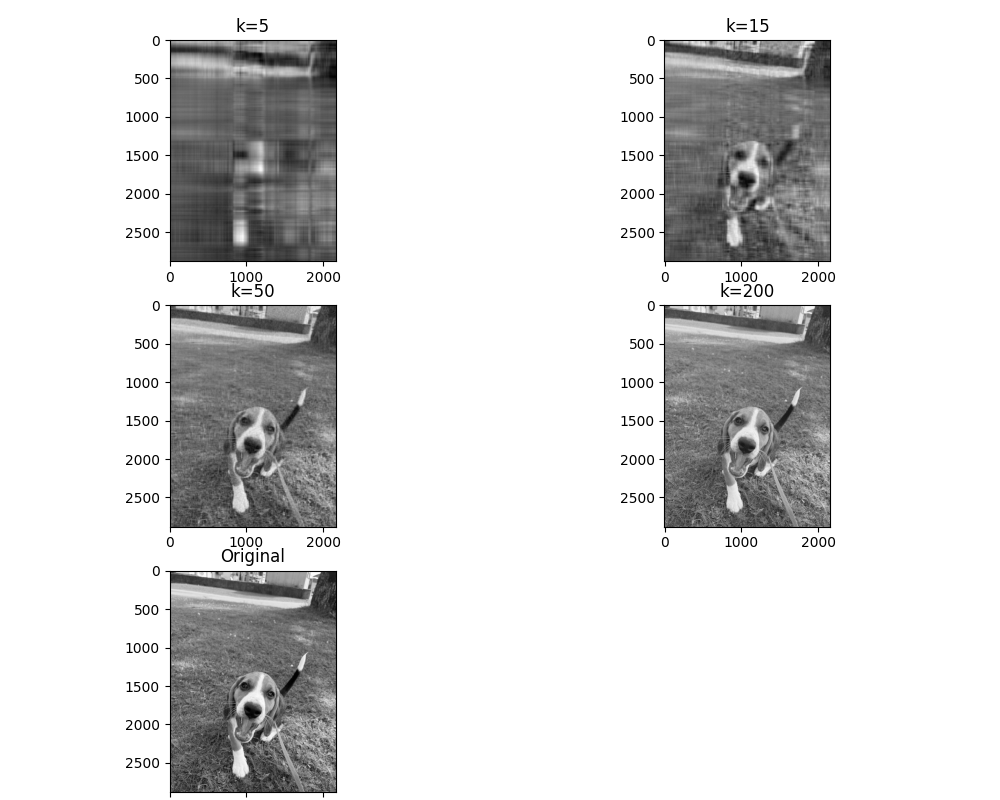
\includegraphics[width=1.4\linewidth]{truncated_images.png}
    \caption{Truncate images of a dog on grass. }
    \label{fig:placeholder}
\end{figure}

\subsection{b)}

Here are the singular values, plotted linearly and logarithmically:

\begin{figure}
    \centering
    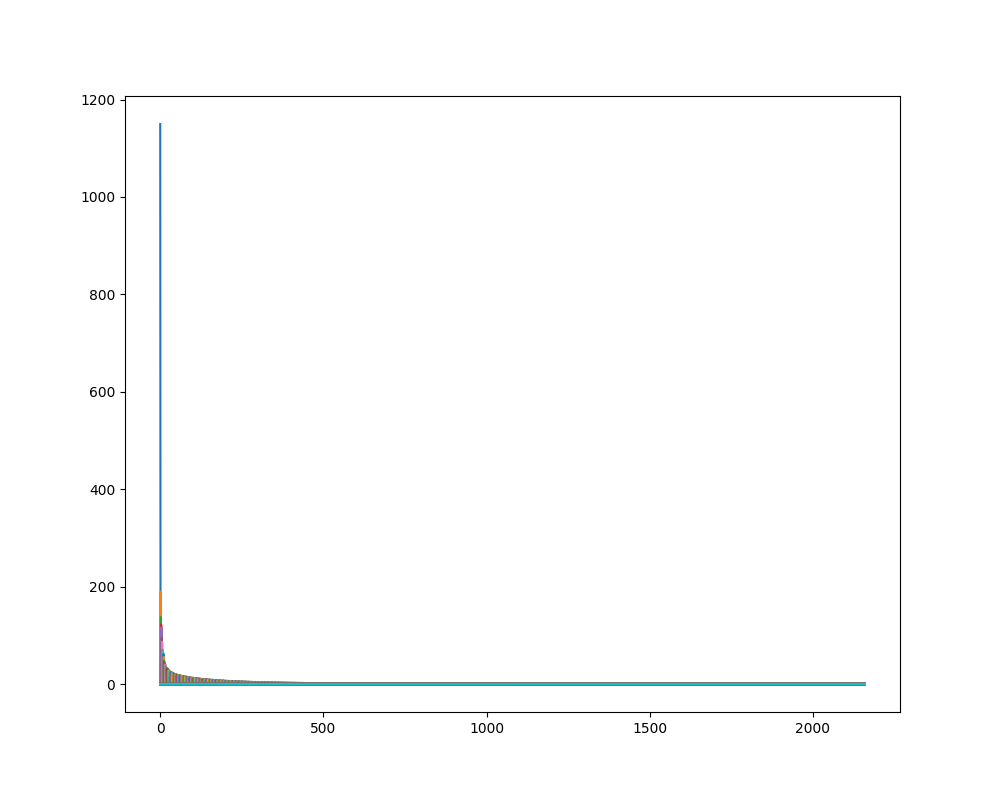
\includegraphics[width=1\linewidth]{singular_values_linear.png}
    \caption{The linear plot.}
    \label{fig:placeholder}
\end{figure}

\begin{figure}[H]
    \centering
    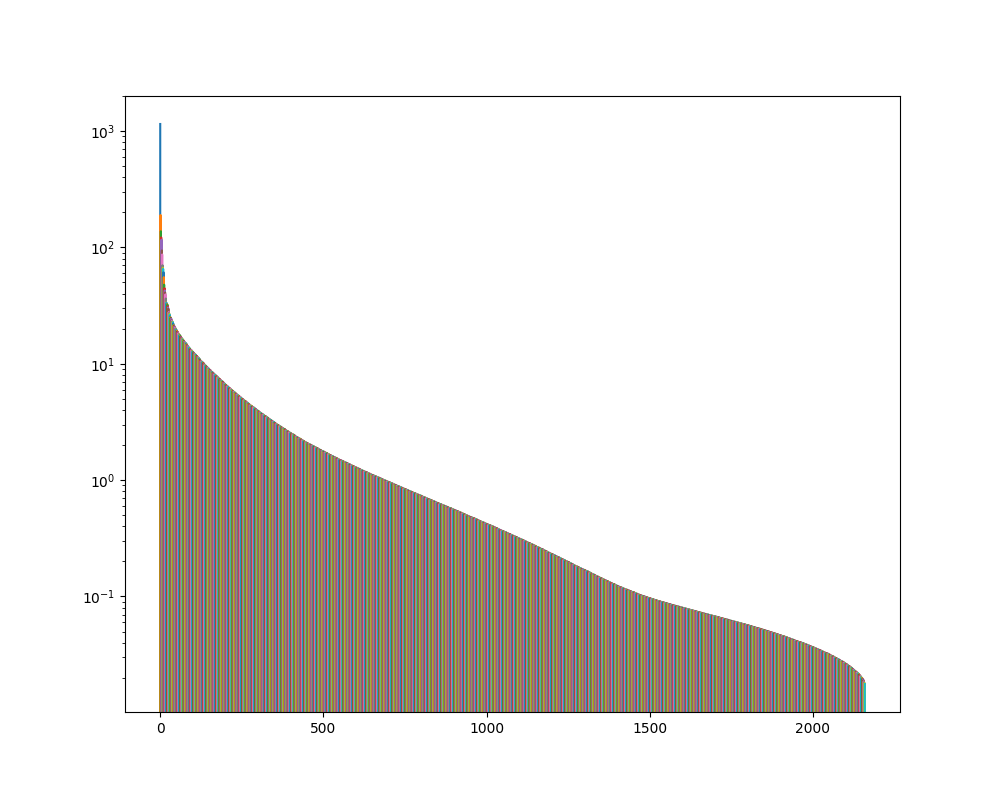
\includegraphics[width=1\linewidth]{singular_values_log.png}
    \caption{The logarithm plot.}
    \label{fig:placeholder}
\end{figure}

It is clear by looking at the plots that the first few singular values hold almost al of the information.

\subsection{c)}

Here are the errors at our choices of $k$:

\begin{table}[H]
  \centering
  \caption{Error as a function of $k$.}
  \label{tab:error-k}
  \begin{tabular}{rr}
    \toprule
    $k$ & Error \\
    \midrule
    5   & 0.251309 \\
    15  & 0.185715 \\
    50  & 0.131520 \\
    200 & 0.055895 \\
    \bottomrule
  \end{tabular}
\end{table}

Verifying numerically that 

\begin{equation}
    ||B-B_r||_F^2=\sum_{j=r+1}^{s}\sigma_j^2,\;\;s=\min(p,q)
\end{equation}

\begin{table}[H]
  \centering
  \caption{Numerical verification.}
  \label{tab:verification}
  \begin{tabular}{lr}
    \toprule
    Quantity & Value \\
    \midrule
    Computed value & 25953.128420042 \\
    Expected value & 25953.128420042 \\
    \bottomrule
  \end{tabular}
\end{table}

\subsection{d)}

SVD image comression reduces the size an image takes. This reduction is given by approximately 

\begin{equation}
    k(p+q+1)
\end{equation}

numbers needed for SVD image storage, compared to $pq$ for an uncompressed image. For our choices of $k$, we get 

\begin{table}[H]
  \centering
  \caption{Storage required for the rank-$k$ approximation. The original image stores $6\,220\,800$ numbers.}
  \label{tab:storage}
  \begin{tabular}{rrr}
    \toprule
    $k$ & Numbers stored & Ratio to original (\%) \\
    \midrule
    5   & 25\,205    & 0.4052 \\
    15  & 75\,615    & 1.216  \\
    50  & 252\,050   & 4.052  \\
    200 & 1\,008\,200 & 16.21  \\
    \bottomrule
  \end{tabular}
\end{table}

St $k=200$, we have compressed the image to $1/6$ its original size. This is impressive, since there is little visual difference between the original and the approximation at $k=200$, this is a viable method of image compression, for our image. 

\subsection{e)}

By checking different values of $k$, we found the following values. 

\begin{table}[H]
  \centering
  \caption{Retained Frobenius norm of the rank-$k$ approximation.}
  \label{tab:frobenius}
  \begin{tabular}{rr}
    \toprule
    $k$ & Retained Frobenius norm (\%) \\
    \midrule
    1  & 88.13 \\
    2  & 90.53 \\
    7  & 94.78 \\
    8  & 95.11 \\
    91 & 98.99 \\
    92 & 99.01 \\
    \bottomrule
  \end{tabular}
\end{table}

Here we see that $90\%$ is retained between $k=1$ and $k=2$, $95\%$ is retained between $k=7$ and $k=8$ and $99\%$ is retained between $k=91$ and $k=92$. 
\newline

This does not match our judgement of visual quality. At $k=5$, the image is not recognizable. At $k=15$, you can barely tell that there is a dog in the image. This is due to the first few singular values being much larger than the rest, but the smaller singular values hold all the fine detail. 

\subsection{f)}

I feel that $k=200$ is a good compromise. It only takes about $16\%$ of the size of the original image, and without zoming in, you can barely tell a difference. At $k=200$, we retain about $99.7\%$ of the Frobenius norm, and the error is approximately $0.0559$. This is a least-squares problem because we want to minimize $\min_{rank(C)\leq r}||B-C||_F^2$. 

However, what k is appropriate depends on the size and contents of the image. 
Images with a smooth gradient, require a lower K, and larger images have a much better storage ratio at higher Ks. So a large image of a fractal would be good with a large K. However a small image of sunset, would be best with a small K. Images of with just one or mostly one color have strange behaviour. 


\end{document}